\section{introduction}
\label{submission}

\begin{figure}[ht]
  \vskip 0.2in
  \begin{center}
  \centerline{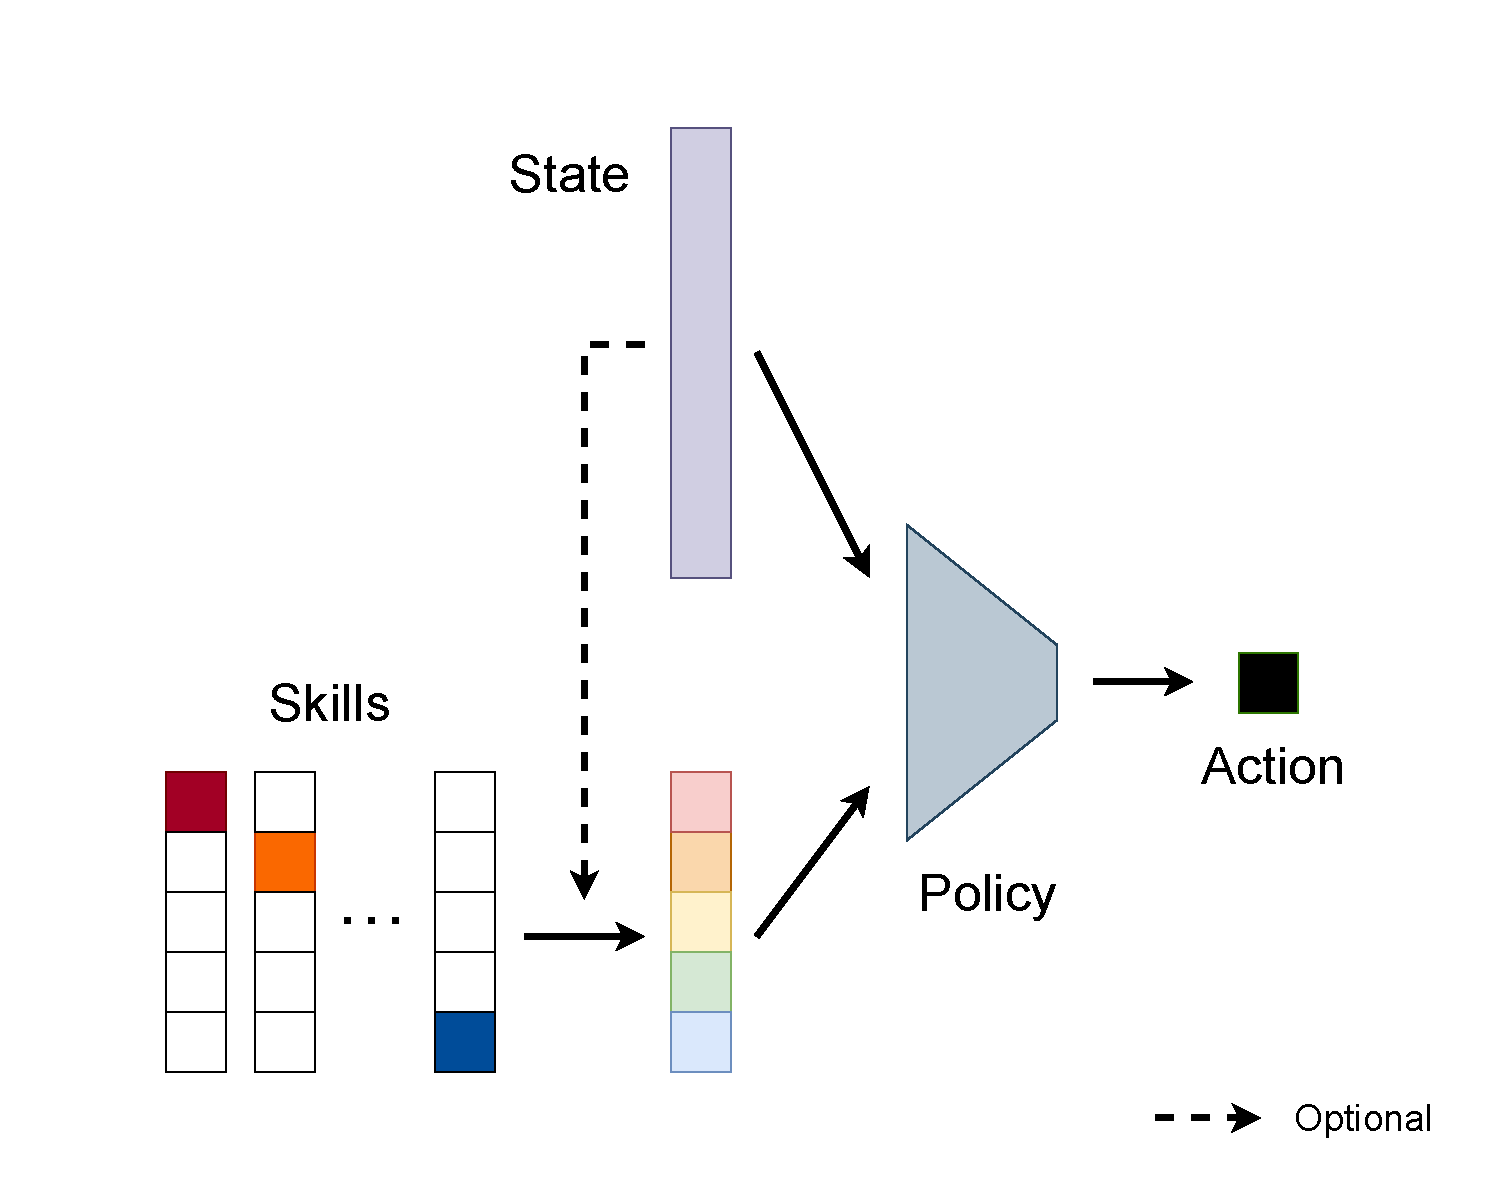
\includegraphics[width=\columnwidth]{Figures/figure_diagram.pdf}}
  \caption{Overview of methods to mix a set of learned skills in fine-tuning phase. It is optional whether the current state affects how the skills combine together.}
  \label{overview}
  \end{center}
  \vskip -0.2in
\end{figure}

Unsupervised learning for deep reinforcement learning (DRL) is challenging in the sense that an agent should interact with the world and collect data to obtain useful information without explicit reward.
In the pretraining step, an agent gathers information from the environment and learns representations of visited states, dynamics, and behaviors.
When the downstream tasks are given, the agent has to quickly adapt to them leveraging those representations.
Recent works have shown that skill discovery is a promising way to learn diverse behaviors which potentially help the agent achieve a goal \cite{salge2014empowerment, gregor2016variational, eysenbach2018diversity}.

Although the agent could learn diverse skills, it is not obvious at a glance how the agent manages them to solve a downstream task since the agent has to efficiently and effectively handle multiple policies while the agent has just one policy to control in a typical reinforcement learning framework.
DIAYN\cite{eysenbach2018diversity} suggested testing all skills in downstream tasks. However, this is very sample-inefficient.
The recent work \cite{laskin2021urlb} which evaluated a variety of unsupervised RL algorithms in locomotion environments, uniformly sampled skill for every episdode even at the finetuning phase.
This leads to significant performance degradation and naturally DIAYN showed poor performance compared to other algorithms according to their work.

Instead of exhaustive skill search nor naive skill sampling, we propose two skill searching methodsin a sample efficient manner.
Both method evaluates the importance of each skill, but the first evaluates the importance of a skill in a state-agnostic way
while the second evaluates the importance of a skill in a state-aware way.
The first method adds tens of parameters($\sim skilldim$) to help agent learn the importance of each skill. With these simple adjustments, the agent can create a policy that considers all skills and achieve good performance in a sample efficient way.
The second method is to add a neural net module that evaluates  skill importance differently according to the input state.
This method has a smoother running curve than the first method, but the final performance is better.
What is noteworthy here is that we use the weight of DIAYN module from the pretraining phase.
During pretraining, the DIAYN module predicted which skill was used when given the state. We thought that this state to skill mapping learning process would be helpful when finetuning.
As expected, with these pretrain weights, the state-aware importance predictor achieved higher performance in a more sample efficient manner.

Moreover, we particularly were curious on whether the agent can acquire the ability to use a combination of several skills rather than just using one skill.
We often see cases where smart communities see the same event from different perspectives and benefit more through combination of perspectives.
As illustrated in \cref*{fig:skill_as_perspective},
when using different skill, different skill weigth vector is used while the transformed state vector remains same regardless of which skill is used.
We interpret this skill weight vector as agent's perspectives. The agent could interprete incoming state differently by adding different skill weight vector.
What we are curious about is whether combining these skills which is adding several skill weight vector to the transformed state vector would happen when the agent is allowed to.
Unfortunately, even when the model performed well, we couldn't observe combination of skills.
Perhaps this is the task was not difficult enough to require a combination of skills.
However, if the task becomes difficult, we expect skill combination will be needed and we leave this left as further work.
\begin{figure}[ht]
  \vskip 0.2in
  \begin{center}
  \centerline{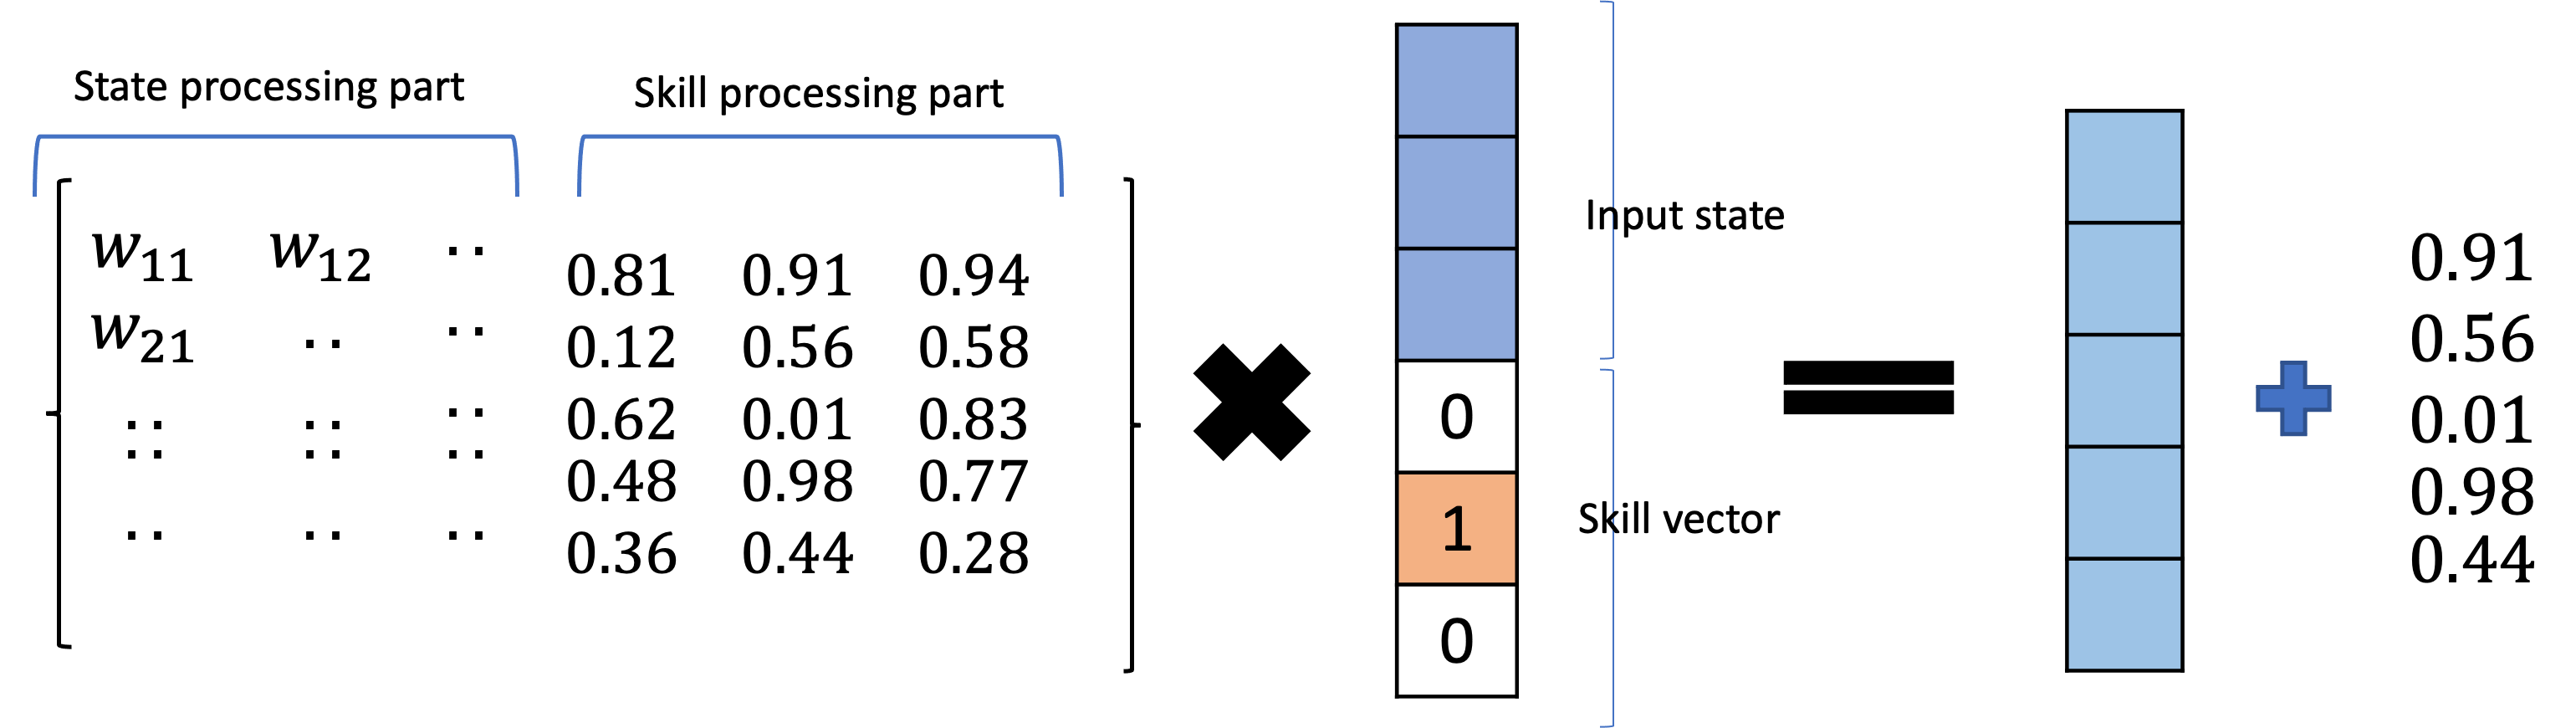
\includegraphics[width=\columnwidth]{Figures/state-skill-decomposition.png}}
  \caption{The Agent is using second skill weight vector to interprete the input state. We inspect combining first and third skill weight vector could contribute to better learning.}
  \label{fig:skill_as_perspective}
  \end{center}
  \vskip -0.2in
\end{figure}

% Our main contribution is to emphasize the importance of fine-tuning in skill discovery by showing the finetuning method can affect the final score a lot for each task.
% We also propose a simple but powerful finetune method utilizing every learned skill.

Our contribution is to introduce a method in which the agent can determine the importance of each skill by itself.
Two methods are presented, a state-agnostic method that can quickly achieve performance above a certain level, and a state-aware method that is slightly slower but more powerful.
In particular, in the second method, the sample-efficiency was increased by using the weight of the DIAYN discriminator used during pretraining, and the final performance was further improved.
